\section{objloader  Class Reference}
\label{classobjloader}\index{objloader@{objloader}}
Parse in .obj's. 


{\tt \#include $<$objloader.hpp$>$}

Inheritance diagram for objloader::\begin{figure}[H]
\begin{center}
\leavevmode
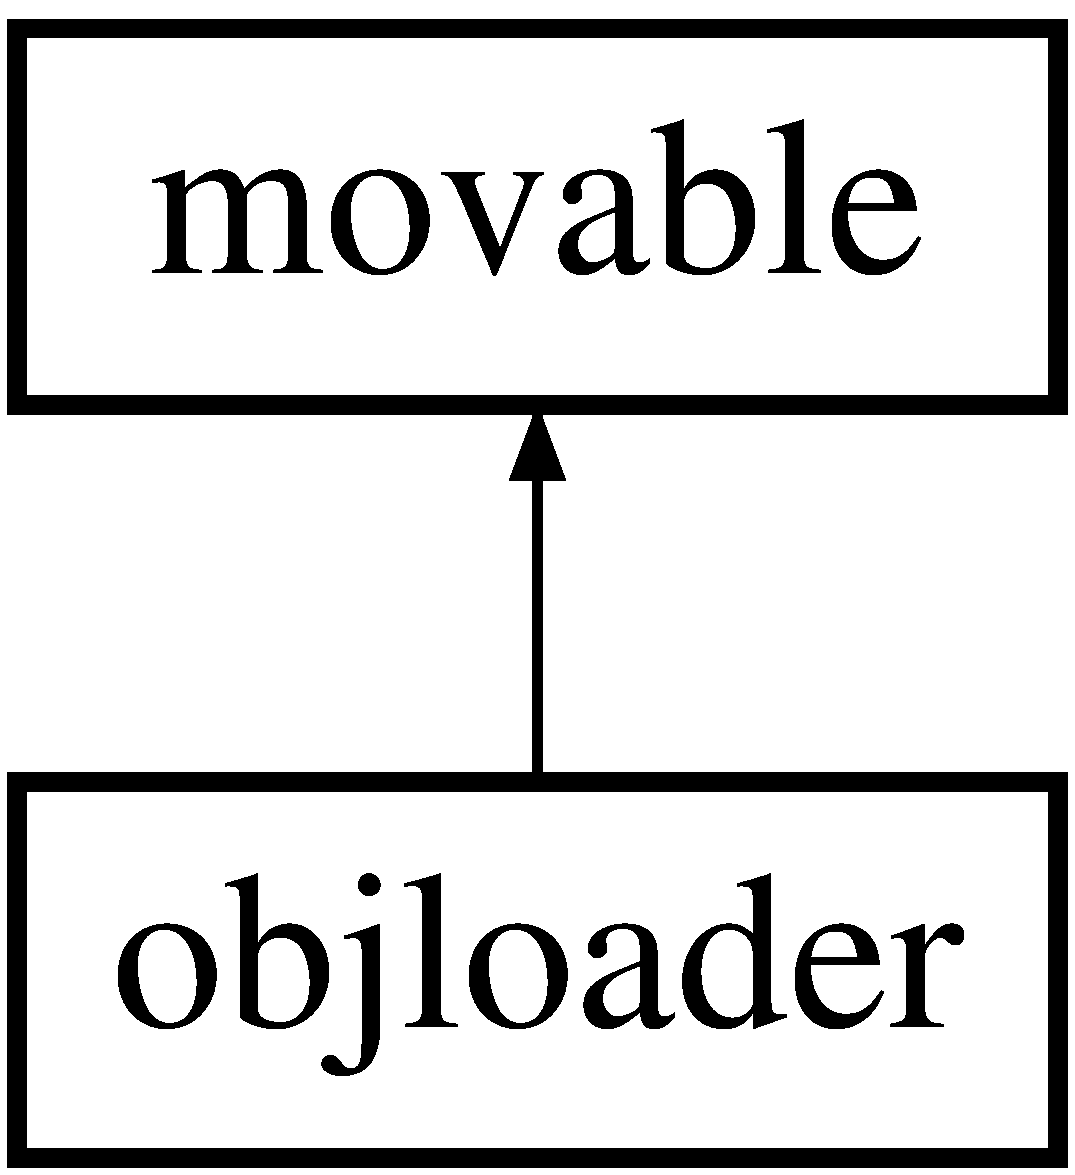
\includegraphics[height=2cm]{classobjloader}
\end{center}
\end{figure}
\subsection*{Public Methods}
\begin{CompactItemize}
\item 
\index{objloader@{objloader}!objloader@{objloader}}\index{objloader@{objloader}!objloader@{objloader}}
{\bf objloader} ()\label{classobjloader_a0}

\item 
\index{objloader@{objloader}!objloader@{objloader}}\index{objloader@{objloader}!objloader@{objloader}}
{\bf objloader} (string obj\-File, float STEP, string subdir=\char`\"{}\char`\"{})\label{classobjloader_a1}

\item 
\index{~objloader@{$\sim$objloader}!objloader@{objloader}}\index{objloader@{objloader}!~objloader@{$\sim$objloader}}
{\bf $\sim$objloader} ()\label{classobjloader_a2}

\item 
\index{load@{load}!objloader@{objloader}}\index{objloader@{objloader}!load@{load}}
bool {\bf load} (string obj\-File)\label{classobjloader_a3}

\begin{CompactList}\small\item\em Load .obj file.\item\end{CompactList}\item 
\index{process@{process}!objloader@{objloader}}\index{objloader@{objloader}!process@{process}}
void {\bf process} (string line)\label{classobjloader_a4}

\begin{CompactList}\small\item\em Parse each line of .obj file.\item\end{CompactList}\item 
\index{loadMtl@{loadMtl}!objloader@{objloader}}\index{objloader@{objloader}!loadMtl@{load\-Mtl}}
void {\bf load\-Mtl} (string mtl\-File)\label{classobjloader_a5}

\begin{CompactList}\small\item\em Parse .mtl file specified in .obj file.\item\end{CompactList}\item 
\index{processMtl@{processMtl}!objloader@{objloader}}\index{objloader@{objloader}!processMtl@{process\-Mtl}}
void {\bf process\-Mtl} (string line, {\bf material} $\ast$mtl)\label{classobjloader_a6}

\begin{CompactList}\small\item\em Parse each line of .mtl file into {\bf material} {\rm (p.\,\pageref{classmaterial})} objects.\item\end{CompactList}\item 
\index{matchMtl@{matchMtl}!objloader@{objloader}}\index{objloader@{objloader}!matchMtl@{match\-Mtl}}
bool {\bf match\-Mtl} (unsigned \&index, string name)\label{classobjloader_a7}

\begin{CompactList}\small\item\em Match specified {\bf material} {\rm (p.\,\pageref{classmaterial})} to loaded materials.\item\end{CompactList}\item 
\index{setMass@{setMass}!objloader@{objloader}}\index{objloader@{objloader}!setMass@{set\-Mass}}
void {\bf set\-Mass} (float new\-Mass)\label{classobjloader_a8}

\begin{CompactList}\small\item\em Change or initialize total mass.\item\end{CompactList}\item 
\index{draw@{draw}!objloader@{objloader}}\index{objloader@{objloader}!draw@{draw}}
void {\bf draw} (void)\label{classobjloader_a9}

\item 
\index{update@{update}!objloader@{objloader}}\index{objloader@{objloader}!update@{update}}
void {\bf update} (void)\label{classobjloader_a10}

\begin{CompactList}\small\item\em Does nothing currently, put scripted movements here.\item\end{CompactList}\item 
\index{operator=@{operator=}!objloader@{objloader}}\index{objloader@{objloader}!operator=@{operator=}}
objloader \& {\bf operator=} (const objloader \&obj1)\label{classobjloader_a11}

\item 
\index{getBoundingBox@{getBoundingBox}!objloader@{objloader}}\index{objloader@{objloader}!getBoundingBox@{get\-Bounding\-Box}}
void {\bf get\-Bounding\-Box} (void)\label{classobjloader_a12}

\end{CompactItemize}
\subsection*{Public Attributes}
\begin{CompactItemize}
\item 
\index{success@{success}!objloader@{objloader}}\index{objloader@{objloader}!success@{success}}
bool {\bf success}\label{classobjloader_m0}

\item 
\index{counter@{counter}!objloader@{objloader}}\index{objloader@{objloader}!counter@{counter}}
int {\bf counter}\label{classobjloader_m1}

\begin{CompactList}\small\item\em For scripted movements, unused currently.\item\end{CompactList}\item 
\index{vertices@{vertices}!objloader@{objloader}}\index{objloader@{objloader}!vertices@{vertices}}
std::vector$<$ {\bf vector3f} $>$ {\bf vertices}\label{classobjloader_m2}

\item 
\index{normals@{normals}!objloader@{objloader}}\index{objloader@{objloader}!normals@{normals}}
std::vector$<$ {\bf vector3f} $>$ {\bf normals}\label{classobjloader_m3}

\item 
\index{mtls@{mtls}!objloader@{objloader}}\index{objloader@{objloader}!mtls@{mtls}}
std::vector$<$ {\bf material} $\ast$ $>$ {\bf mtls}\label{classobjloader_m4}

\item 
\index{listNum@{listNum}!objloader@{objloader}}\index{objloader@{objloader}!listNum@{list\-Num}}
int {\bf list\-Num}\label{classobjloader_m5}

\begin{CompactList}\small\item\em Which opengl call list.\item\end{CompactList}\item 
\index{iStack@{iStack}!objloader@{objloader}}\index{objloader@{objloader}!iStack@{i\-Stack}}
std::vector$<$ {\bf vector3f} $>$ {\bf i\-Stack}\label{classobjloader_m6}

\item 
\index{surface@{surface}!objloader@{objloader}}\index{objloader@{objloader}!surface@{surface}}
std::vector$<$ {\bf vector3f} $>$ {\bf surface}\label{classobjloader_m7}

\item 
\index{centerOfMass@{centerOfMass}!objloader@{objloader}}\index{objloader@{objloader}!centerOfMass@{center\-Of\-Mass}}
{\bf vector3f} {\bf center\-Of\-Mass}\label{classobjloader_m8}

\item 
\index{translucent@{translucent}!objloader@{objloader}}\index{objloader@{objloader}!translucent@{translucent}}
bool {\bf translucent}\label{classobjloader_m9}

\end{CompactItemize}


\subsection{Detailed Description}
Parse in .obj's.

I could do more parsers for other formats but .objs fit all my needs for now (I'll need my own format most likely).

Perhaps I should further separate obj loading from the physics operations for finding the interior points and so forth. 



The documentation for this class was generated from the following files:\begin{CompactItemize}
\item 
{\bf objloader.hpp}\item 
objloader.cpp\end{CompactItemize}
